\documentclass[conference]{IEEEtran}
\IEEEoverridecommandlockouts

% *** CITATION PACKAGES ***
%
\usepackage{cite}
% cite.sty was written by Donald Arseneau
% V1.6 and later of IEEEtran pre-defines the format of the cite.sty package
% \cite{} output to follow that of IEEE. Loading the cite package will
% result in citation numbers being automatically sorted and properly
% "compressed/ranged". e.g., [1], [9], [2], [7], [5], [6] without using
% cite.sty will become [1], [2], [5]--[7], [9] using cite.sty. cite.sty's
% \cite will automatically add leading space, if needed. Use cite.sty's
% noadjust option (cite.sty V3.8 and later) if you want to turn this off.
% cite.sty is already installed on most LaTeX systems. Be sure and use
% version 4.0 (2003-05-27) and later if using hyperref.sty. cite.sty does
% not currently provide for hyperlinked citations.
% The latest version can be obtained at:
% http://www.ctan.org/tex-archive/macros/latex/contrib/cite/
% The documentation is contained in the cite.sty file itself.

% *** GRAPHICS RELATED PACKAGES ***
%
\ifCLASSINFOpdf
  \usepackage[pdftex]{graphicx}
  % declare the path(s) where your graphic files are
  % \graphicspath{{../pdf/}{../jpeg/}}
  \graphicspath{{images/}}
  % and their extensions so you won't have to specify these with
  % every instance of \includegraphics
  \DeclareGraphicsExtensions{.jpeg,.png}
\else
  % or other class option (dvipsone, dvipdf, if not using dvips). graphicx
  % will default to the driver specified in the system graphics.cfg if no
  % driver is specified.
  % \usepackage[dvips]{graphicx}
  % declare the path(s) where your graphic files are
  % \graphicspath{{../eps/}}
  % and their extensions so you won't have to specify these with
  % every instance of \includegraphics
  % \DeclareGraphicsExtensions{.eps}
\fi
% graphicx was written by David Carlisle and Sebastian Rahtz. It is
% required if you want graphics, photos, etc. graphicx.sty is already
% installed on most LaTeX systems. The latest version and documentation can
% be obtained at: 
% http://www.ctan.org/tex-archive/macros/latex/required/graphics/
% Another good source of documentation is "Using Imported Graphics in
% LaTeX2e" by Keith Reckdahl which can be found as epslatex.ps or
% epslatex.pdf at: http://www.ctan.org/tex-archive/info/
%
% latex, and pdflatex in dvi mode, support graphics in encapsulated
% postscript (.eps) format. pdflatex in pdf mode supports graphics
% in .pdf, .jpeg, .png and .mps (metapost) formats. Users should ensure
% that all non-photo figures use a vector format (.eps, .pdf, .mps) and
% not a bitmapped formats (.jpeg, .png). IEEE frowns on bitmapped formats
% which can result in "jaggedy"/blurry rendering of lines and letters as
% well as large increases in file sizes.
%
% You can find documentation about the pdfTeX application at:
% http://www.tug.org/applications/pdftex

% *** MATH PACKAGES ***
%
%\usepackage[cmex10]{amsmath}
% A popular package from the American Mathematical Society that provides
% many useful and powerful commands for dealing with mathematics. If using
% it, be sure to load this package with the cmex10 option to ensure that
% only type 1 fonts will utilized at all point sizes. Without this option,
% it is possible that some math symbols, particularly those within
% footnotes, will be rendered in bitmap form which will result in a
% document that can not be IEEE Xplore compliant!
%
% Also, note that the amsmath package sets \interdisplaylinepenalty to 10000
% thus preventing page breaks from occurring within multiline equations. Use:
%\interdisplaylinepenalty=2500
% after loading amsmath to restore such page breaks as IEEEtran.cls normally
% does. amsmath.sty is already installed on most LaTeX systems. The latest
% version and documentation can be obtained at:
% http://www.ctan.org/tex-archive/macros/latex/required/amslatex/math/

% *** SPECIALIZED LIST PACKAGES ***
%
%\usepackage{algorithmic}
% algorithmic.sty was written by Peter Williams and Rogerio Brito.
% This package provides an algorithmic environment fo describing algorithms.
% You can use the algorithmic environment in-text or within a figure
% environment to provide for a floating algorithm. Do NOT use the algorithm
% floating environment provided by algorithm.sty (by the same authors) or
% algorithm2e.sty (by Christophe Fiorio) as IEEE does not use dedicated
% algorithm float types and packages that provide these will not provide
% correct IEEE style captions. The latest version and documentation of
% algorithmic.sty can be obtained at:
% http://www.ctan.org/tex-archive/macros/latex/contrib/algorithms/
% There is also a support site at:
% http://algorithms.berlios.de/index.html
% Also of interest may be the (relatively newer and more customizable)
% algorithmicx.sty package by Szasz Janos:
% http://www.ctan.org/tex-archive/macros/latex/contrib/algorithmicx/


% *** ALIGNMENT PACKAGES ***
%
%\usepackage{array}
% Frank Mittelbach's and David Carlisle's array.sty patches and improves
% the standard LaTeX2e array and tabular environments to provide better
% appearance and additional user controls. As the default LaTeX2e table
% generation code is lacking to the point of almost being broken with
% respect to the quality of the end results, all users are strongly
% advised to use an enhanced (at the very least that provided by array.sty)
% set of table tools. array.sty is already installed on most systems. The
% latest version and documentation can be obtained at:
% http://www.ctan.org/tex-archive/macros/latex/required/tools/


%\usepackage{mdwmath}
%\usepackage{mdwtab}
% Also highly recommended is Mark Wooding's extremely powerful MDW tools,
% especially mdwmath.sty and mdwtab.sty which are used to format equations
% and tables, respectively. The MDWtools set is already installed on most
% LaTeX systems. The lastest version and documentation is available at:
% http://www.ctan.org/tex-archive/macros/latex/contrib/mdwtools/


% IEEEtran contains the IEEEeqnarray family of commands that can be used to
% generate multiline equations as well as matrices, tables, etc., of high
% quality.


%\usepackage{eqparbox}
% Also of notable interest is Scott Pakin's eqparbox package for creating
% (automatically sized) equal width boxes - aka "natural width parboxes".
% Available at:
% http://www.ctan.org/tex-archive/macros/latex/contrib/eqparbox/





% *** SUBFIGURE PACKAGES ***
%\usepackage[tight,footnotesize]{subfigure}
% subfigure.sty was written by Steven Douglas Cochran. This package makes it
% easy to put subfigures in your figures. e.g., "Figure 1a and 1b". For IEEE
% work, it is a good idea to load it with the tight package option to reduce
% the amount of white space around the subfigures. subfigure.sty is already
% installed on most LaTeX systems. The latest version and documentation can
% be obtained at:
% http://www.ctan.org/tex-archive/obsolete/macros/latex/contrib/subfigure/
% subfigure.sty has been superceeded by subfig.sty.



%\usepackage[caption=false]{caption}
%\usepackage[font=footnotesize]{subfig}
% subfig.sty, also written by Steven Douglas Cochran, is the modern
% replacement for subfigure.sty. However, subfig.sty requires and
% automatically loads Axel Sommerfeldt's caption.sty which will override
% IEEEtran.cls handling of captions and this will result in nonIEEE style
% figure/table captions. To prevent this problem, be sure and preload
% caption.sty with its "caption=false" package option. This is will preserve
% IEEEtran.cls handing of captions. Version 1.3 (2005/06/28) and later 
% (recommended due to many improvements over 1.2) of subfig.sty supports
% the caption=false option directly:
%\usepackage[caption=false,font=footnotesize]{subfig}
%
% The latest version and documentation can be obtained at:
% http://www.ctan.org/tex-archive/macros/latex/contrib/subfig/
% The latest version and documentation of caption.sty can be obtained at:
% http://www.ctan.org/tex-archive/macros/latex/contrib/caption/




% *** FLOAT PACKAGES ***
%
%\usepackage{fixltx2e}
% fixltx2e, the successor to the earlier fix2col.sty, was written by
% Frank Mittelbach and David Carlisle. This package corrects a few problems
% in the LaTeX2e kernel, the most notable of which is that in current
% LaTeX2e releases, the ordering of single and double column floats is not
% guaranteed to be preserved. Thus, an unpatched LaTeX2e can allow a
% single column figure to be placed prior to an earlier double column
% figure. The latest version and documentation can be found at:
% http://www.ctan.org/tex-archive/macros/latex/base/



%\usepackage{stfloats}
% stfloats.sty was written by Sigitas Tolusis. This package gives LaTeX2e
% the ability to do double column floats at the bottom of the page as well
% as the top. (e.g., "\begin{figure*}[!b]" is not normally possible in
% LaTeX2e). It also provides a command:
%\fnbelowfloat
% to enable the placement of footnotes below bottom floats (the standard
% LaTeX2e kernel puts them above bottom floats). This is an invasive package
% which rewrites many portions of the LaTeX2e float routines. It may not work
% with other packages that modify the LaTeX2e float routines. The latest
% version and documentation can be obtained at:
% http://www.ctan.org/tex-archive/macros/latex/contrib/sttools/
% Documentation is contained in the stfloats.sty comments as well as in the
% presfull.pdf file. Do not use the stfloats baselinefloat ability as IEEE
% does not allow \baselineskip to stretch. Authors submitting work to the
% IEEE should note that IEEE rarely uses double column equations and
% that authors should try to avoid such use. Do not be tempted to use the
% cuted.sty or midfloat.sty packages (also by Sigitas Tolusis) as IEEE does
% not format its papers in such ways.

% *** PDF, URL AND HYPERLINK PACKAGES ***
%
\usepackage{url}
% url.sty was written by Donald Arseneau. It provides better support for
% handling and breaking URLs. url.sty is already installed on most LaTeX
% systems. The latest version can be obtained at:
% http://www.ctan.org/tex-archive/macros/latex/contrib/misc/
% Read the url.sty source comments for usage information. Basically,
% \url{my_url_here}.


% *** Do not adjust lengths that control margins, column widths, etc. ***
% *** Do not use packages that alter fonts (such as pslatex).         ***
% There should be no need to do such things with IEEEtran.cls V1.6 and later.
% (Unless specifically asked to do so by the journal or conference you plan
% to submit to, of course. )


% correct bad hyphenation here
\hyphenation{op-tical net-works semi-conduc-tor}

% Drop caps with \lettrine
\usepackage{type1cm}
\usepackage{lettrine}

 % \raggedbottom
\begin{document}
\title{\uppercase{SnipR}: Complementing Code Search with Code Retargeting Capabilities}

\author{\IEEEauthorblockN{Huascar A. Sanchez\thanks{Advisor: Prof. Jim Whitehead, University of California, Santa Cruz}}
\IEEEauthorblockA{
Computer Science Department\\University of California, Santa Cruz\\
Santa Cruz, CA 95060\\
hsanchez@cs.ucsc.edu}}

% conference papers do not typically use \thanks and this command
% is locked out in conference mode. If really needed, such as for
% the acknowledgment of grants, issue a \IEEEoverridecommandlockouts
% after \documentclass

% for over three affiliations, or if they all won't fit within the width
% of the page, use this alternative format:
% 
%\author{\IEEEauthorblockN{Michael Shell\IEEEauthorrefmark{1},
%Homer Simpson\IEEEauthorrefmark{2},
%James Kirk\IEEEauthorrefmark{3}, 
%Montgomery Scott\IEEEauthorrefmark{3} and
%Eldon Tyrell\IEEEauthorrefmark{4}}
%\IEEEauthorblockA{\IEEEauthorrefmark{1}School of Electrical and Computer Engineering\\
%Georgia Institute of Technology,
%Atlanta, Georgia 30332--0250\\ Email: see http://www.michaelshell.org/contact.html}
%\IEEEauthorblockA{\IEEEauthorrefmark{2}Twentieth Century Fox, Springfield, USA\\
%Email: homer@thesimpsons.com}
%\IEEEauthorblockA{\IEEEauthorrefmark{3}Starfleet Academy, San Francisco, California 96678-2391\\
%Telephone: (800) 555--1212, Fax: (888) 555--1212}
%\IEEEauthorblockA{\IEEEauthorrefmark{4}Tyrell Inc., 123 Replicant Street, Los Angeles, California 90210--4321}}

% use for special paper notices
%\IEEEspecialpapernotice{(Invited Paper)}




% make the title area
\maketitle

\begin{abstract}
%\boldmath
In a typical code search process, developers are given no guidance as to which result may be a best fit for their code in progress, beyond the use of ranking values. Tool support for predetermining whether a ranked searched source (e.g., example code) is a best fit for one's code is still non-existent. This makes the integration of such example code needlessly costly and difficult. This paper introduces a new approach in search-oriented architecture, called the Snippet Retargeting Model or simply \uppercase{SnipR}. \uppercase{SnipR} addresses the aforementioned limitation by complementing code search with code retargeting capabilities (i.e., code manipulation). The intent of these capabilities is to expedite the process of determining if a source code is a best fit--- i.e., suitable---directly from the search interface. 
\end{abstract}
% IEEEtran.cls defaults to using nonbold math in the Abstract.
% This preserves the distinction between vectors and scalars. However,
% if the conference you are submitting to favors bold math in the abstract,
% then you can use LaTeX's standard command \boldmath at the very start
% of the abstract to achieve this. Many IEEE journals/conferences frown on
% math in the abstract anyway.

% no keywords


% For peer review papers, you can put extra information on the cover
% page as needed:
% \ifCLASSOPTIONpeerreview
% \begin{center} \bfseries EDICS Category: 3-BBND \end{center}
% \fi
%
% For peerreview papers, this IEEEtran command inserts a page break and
% creates the second title. It will be ignored for other modes.
\IEEEpeerreviewmaketitle

\section{Research Problem and Solution Outline}
\label{sec:intro}
\lettrine[lraise=0.1, nindent=0em, slope=-.5em]{T} {he recent rise} of Internet-scale code search engines---e.g., Seahawk~\cite{Bacchelli:2012dl}, Portfolio~\cite{McMillan:2011wq}, Sourcerer~\cite{Bajracharya:2006vn}, Koders~\footnote{\url{http://www.koders.com}}---has catapulted search-driven development from backwater to ubiquity, and given rise to an active research community focused on this phenomena~\cite{Bajracharya:2009fj, Bajracharya:2010iy, Bajracharya:2011kw}. The increased prevalence of such engines has given search-driven development more diverse sources of information---e.g., from open sourced code to code snippets from StackOverflow~\footnote{\url{http://www.stackoverflow.com}}---and a more open platform---the Internet~\cite{GallardoValencia:2009gr, GallardoValencia:2010ij, Ying:2012tr}. This new condition has enabled developers to build applications opportunistically by iteratively finding, combining, and reusing online source code~\cite{Brandt:2008wi, Brandt:2009jb, Ying:2012tr}. This opportunistic way of building applications is not easy because searched sources are large, in most cases unsuitable, and quite often unrelated~\cite{GallardoValencia:2009gr}. Consequently, if search-driven development were to be established as best practice, then the time involved in deciding the best search result(s) to reuse must be minimized.

Previously published work has tried to tackle the above problem from different directions. Two of these directions are the most popular. One direction focuses entirely on enhancing search technology~\cite{Bajracharya:2010um, Gysin:2010kt, Mandelin:2005uj, McMillan:2011cm, McMillan:2012dj}, while the other direction focuses on coupling Web search and community-based knowledge with IDEs~\cite{Bacchelli:2012dl, Brandt:2010tp, Hartmann:2010hx, Hoffmann:2007wo, Wightman:2012gc}. Although these directions focus on addressing the trustability and relevance of search results, none of them adequately address the \emph{suitability} of these results. In other words, developers are given no guidance as to which result may be a best fit for their code in progress, beyond the existing ranking values. Precisely, developers still have to \emph{manually} mine and try all these ranked results before they could possibly realize their usefulness---or uselessness. This limitation is one of the reasons why search-driven development is so cumbersome, and ultimately can be a drain on one of the most precious resources in software development: time. 

To alleviate the problem imposed by the above limitation, I propose a new approach in search-oriented architecture, called the Snippet Retargeting Model or simply \uppercase{SnipR}. \uppercase{SnipR} complements code search with code retargeting capabilities---i.e., code manipulation---(See Figure~\ref{fig:retargeting}). The intent of these capabilities is to expedite the process of determining if a source code is a best fit; i.e., suitable. These capabilities are embedded within the \emph{query processing} step of a code search engine in order to automatically modify retrieved source code. Each query issued by a developer is interpreted by the query engine not only as a request for a particular result set, but also as a command to retarget relevant bodies of code in that set; e.g., to modify a retrieved example to use an alternative API. This offers two important advantages. If the developer is retargeting the source in advance, then the evaluation results of retargeted examples are available immediately, which saves valuable human time searching for an appropriate example code. If the developer is choosing what example code to retarget, then the evaluation results can inform the decision, pointing the developer to the best choice. This is an attractive proposition and very different to the directions taken by previous work. It is attractive because one can figure out as early as possible if an example code is appropriate or not. It is different because one can do this without requiring to leave the search interface. The \uppercase{SnipR} approach will be examined by addressing the following research questions:

\begin{itemize}  
\item[RQ1] What kind of \uppercase{SnipR} commands could be invoked directly from the search box?
\item[RQ2] How expensive is it to retarget (part of) examples each time?
\item[RQ3] Where does \uppercase{SnipR} belong within the query processing step of any modern code search engine?
\item[RQ4] How does the time needed to perform a more complete code search task of the SnipR approach compare to the current approaches of code search? 
\end{itemize}

\begin{figure}[!t]
    \centering
    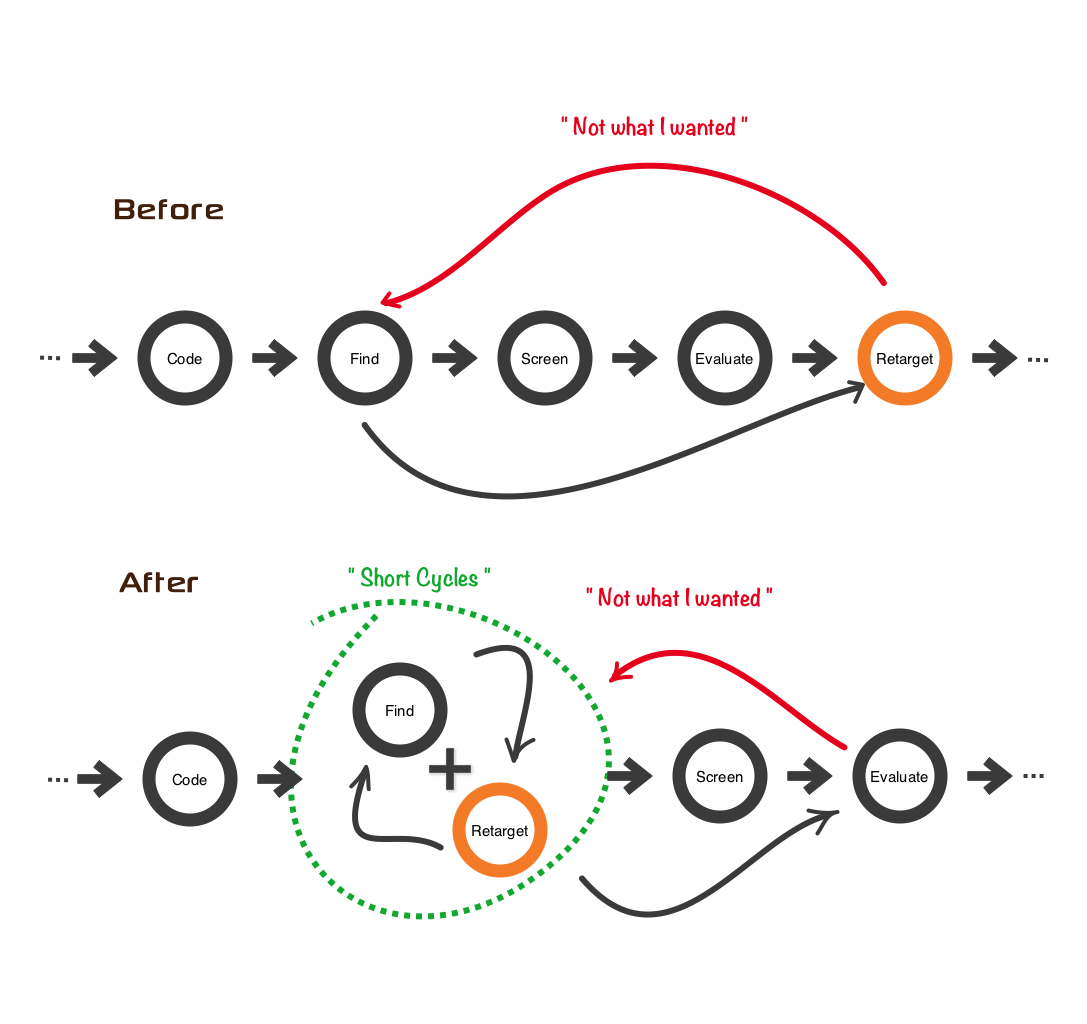
\includegraphics[width=2.8in]{images/searchprocess}
    \caption{Search Process before and with \uppercase{SnipR}. A pre--\uppercase{SnipR} scenario requires effort from the developer to find and select the most promising examples (i.e., screening), and to evaluate each one of them before eventually consuming them (e.g., done with integration) after many code modifications in the IDE. If the resulting code is not the desired code, then the search process is restarted by the developer. In the \uppercase{SnipR} scenario, the developer engages in a virtuous loop where he/she finds and selects only the promising examples that can be retargeted. At this point, the developer would rely on the suitability of these candidates to identify the next course of action.}
    \label{fig:retargeting}
\end{figure}
For RQ1, a command line language for retargeting source code is proposed. This language allows requests for results and retargeting commands to be intermixed or used separately. This feature allows developers to explore potential code changes on the retrieved results. For RQ2, a set of algorithms for learning semantic-preserving code transformations---hereafter called code mappings---from example code is proposed. Once these mappings are learned, the query engine must be able to apply them. Therefore, a set of code retargeting operators well-suited for manipulating example code within query processing is also proposed (RQ2). These operators are proposed to address the application of code mappings. For RQ3, the \uppercase{SnipR} conceptual architecture is realized in a working code search engine. For RQ4, an evaluation of the efficiency of the \uppercase{SnipR} approach vs. existing approaches for code search is performed. 
 % Of the various sources of information developers find on the Web, example code is the most popular choice since they demonstrate how one should use an given API~\cite{Robillard:2009cs}. Tool support for predetermining whether any ranked example code is a best fit for one’s code is still non-existent. Researchers in search-driven development have tackled 

These solutions are the expected contributions in search-driven development and thus in software engineering. All this work is motivated by a grander vision of where the next generation of programming practices and behaviors involving code search could take us. The time is ripe to change the role of code search as a development tool from a mere supporting role to a starring role. 

For the rest of the paper, the focus will shift to the proposed solution to RQ1 (Section~\ref{sec:rq1}), and to a brief description of RQ2, RQ3, and RQ4 in Section~\ref{sec:restqs}. Section~\ref{sec:evaluate} briefly describes a plan for evaluating this work. Section~\ref{sec:progress} outlines the progress to date and Section~\ref{sec:conclude} concludes this paper. 

\section{Proposed Solutions}
\subsection{Designing \uppercase{SnipR} commands that could be invoked directly from the search box (RQ1)}
\label{sec:rq1}
Unpacking this a bit, the key idea is to design a set of retargeting commands that could be invoked from the search box, without losing any sight of the current search goal. This design should balance two inter-related principles: ease of use and generality. To understand what's needed to produce this type of design, I'll turn to the seminal work on sloppy command lines for the Web~\cite{Little:2007dh, Miller:2008ge} and on platform-specific linguistic command lines~\cite{Raskin:2008wb}. Similar to both types of work, the \uppercase{SnipR}'s command line will have flexible syntax requirements. This flexibility offers an important advantage. It allows requests for results and commands to be intermixed---or used separately. The focus of these commands will be on performing code modifications on retrieved example code. A simple but well principled rule will be applied to decide when RQ1 has been completed: there are no longer reasons to change any of the already defined commands. Previous work in command lines for code modifications exist and could be usually seen implemented as plugins in mainstream IDEs, such as Eclipse\footnote{\url{http://www.eclipse.org}} and IntelliJ IDEA\footnote{\url{http://www.jetbrains.com}}. In contrast, with \uppercase{SnipR}, developers will continue to use their Web browser to do these code modifications. 

\subsection{Performing Code Retargeting (RQ2, RQ3, and RQ4)}
\label{sec:restqs}
Code modification---to make code more suited---or retargeting is an operation that can work on a single search result or an entire result set. Therefore, this operation requires that those cases where code mappings can be learned and/or applied are carefully identified. This will prevent any unnecessary work from happening as matched code examples are being returned by the query engine. This requirement will be addressed by developing a set of reliable and cache conscious \uppercase{SnipR} algorithms (RQ2). They should be reliable in the sense of consistently learning code mappings from example code. They should be cache conscious in the sense of exploiting recently read example code if this code must be read again in the future. The output of these algorithms are code mappings that are applied by the query engine when retargeting is needed. In order for the query engine to do that, a set of code retargeting operators well-suited for manipulating example code within query processing must be created (RQ2). These operators should be reliable in the sense of applying learned mappings. Moreover, they should be implemented within the querying processing step of a working code search engine (RQ3). 

In retrospect, if the developer retargets code in advance, then the evaluation results are available immediately, which saves valuable time searching for appropriate example code (See Figure~\ref{fig:retargeting}). By saving this time, the developers will get the work done more quickly (RQ4). This will be possible only if \uppercase{SnipR}'s retargeting operations are efficient, which will be demonstrated by answering RQ2. 

Previous work in adapting code to alternate contexts and/or to new APIs exist. Such work has helped developers with many development tasks, such as adapting example code to new contexts~\cite{Wightman:2012gc} or to new APIs~\cite{Nita:2010en}. This also includes resolving many simple coding errors quickly\footnote{{Quick Fix Scout: \url{https://code.google.com/p/quick-fix-scout/}}, {EUKLAS: \url{http://www.cs.cmu.edu/~euklas}}}, or suggesting ways for correcting compiler and runtime errors~\cite{Hartmann:2010hx}. Unlike \uppercase{SnipR}, any interaction for finding and changing any example code or suggesting solutions to a problem in the developer's code is directly done in the IDE.

\section{Evaluation}
\label{sec:evaluate}

The evaluation methodology to be followed is to validate the \uppercase{SnipR} approach and results through user and lab studies. The tests will be run on \uppercase{SnipR} prototypes in a working code search system, such the Sourcerer\cite{Bajracharya:2006vn} Internet-scale code search engine. The user studies will involve 10 subjects, solicited from a public mailing list at a college campus. The 10 subjects will be also experienced Web users, have some or none programming experience, and could type reasonably well. The use and test of the \uppercase{SnipR} prototype will be done on the basis of a programming problem to be solved; aiming to answer the research questions listed in Section~\ref{sec:intro}. For instance, 

\begin{itemize}  
\item A user study will be performed to test for the expressiveness of the developed command line language. The test attempts to determine how intuitive this language is for end users. The test is also used to determine how this language might be used in daily development activities and to evaluate some of the decisions made on the design of the language's ``intuitively readable commands.'' Each subject will sit at a computer loaded with the a code search system---loaded with \uppercase{SnipR} prototype. Each subject will be directed to a website to receive instructions on how to start using \uppercase{SnipR}. The instructions will indicate that each subject should use only the search box to do any assigned tasks. The instructions will also state a programming problem to be solved: changing a sentiment analysis tool (that uses Twitter API) to use the Facebook API. The data gathered from this test will shed light on learnability, ease of use, and generality of created commands (RQ1).
\item The same user study---previously mentioned---is also used to provide a feel for the speed and accuracy of the  \uppercase{SnipR} algorithms and retargeting operators. Inputs from the user study will be used to derive an average processing time---in terms of learning and applying code mappings from/to example code. It is expected that the processing time varies for input sizes of different lengths. From this, one could guess that the average-case running time is polynomial, but that it is reasonable for relatively small source code (e.g., less than 40 lines of code), such is the case of example code (RQ2). 
\item A lab study will be conducted to gauge the goodness for where in the query processing step the retargeting operators should be implemented. For this lab study three versions of a working code search system will be released. The first version, \uppercase{SnipR}--A, will have these operators implemented inside the interpreter of the command line language. The second version, \uppercase{SnipR}--B, will have these operators nested inside the query engine's existing operators. The third version, \uppercase{SnipR}--C, will have these operators implemented as additional operators of the query engine. This lab attempts to gauge how responsive these operators when facing many different of workloads---i.e., queries or commands issued by a user. This lab is also used to provide a feel for the scalability of these operators (which is expected to be high). The data gathered from this lab will shed light on where \uppercase{SnipR} belongs within the query processing step of any modern code search engine (RQ3). 

\end{itemize}


\section{Progress to Date}
\label{sec:progress}
This work is still at early stages. Work in progress include my advancement to candidacy by the end of this year, and an early design of the command line language for retargeting source code. The development of code retargeting algorithms, the realization of the \uppercase{SnipR} conceptual architecture, and the development of a set of retargeting operators are work that remains.

\section{Conclusion}
\label{sec:conclude}
This paper has introduced \uppercase{SnipR}, an approach that complements code search with code retargeting capabilities. Unlike prior work, the \uppercase{SnipR} enables developers to engage in a virtuous loop where they find and select only the promising example code that can be retargeted. This will minimize the number of iterations in the search process the developer has to go through, since the evaluation step is only dealing with best choices---choices that would be easier to consume later in the IDE. It is envisioned that \uppercase{SnipR} will not be seen as a competitor to any code search systems, but more like a platform. A platform for searching for suitable code.

% references section

% can use a bibliography generated by BibTeX as a .bbl file
% BibTeX documentation can be easily obtained at:
% http://www.ctan.org/tex-archive/biblio/bibtex/contrib/doc/
% The IEEEtran BibTeX style support page is at:
% http://www.michaelshell.org/tex/ieeetran/bibtex/
\bibliographystyle{IEEEtran}
% argument is your BibTeX string definitions and bibliography database(s)
\bibliography{IEEEabrv,icscdocsym}
%
	
\end{document}
